\documentclass[helvetica,english,nologo,notitle,totpages]{europecv2013}
\usepackage[T1]{fontenc}
\usepackage{graphicx}
\usepackage[a4paper,top=1.27cm,left=1cm,right=1cm,bottom=2cm]{geometry}
\usepackage[english]{babel}
\usepackage{bibentry}
\usepackage{natbib}

\renewcommand{\ttdefault}{phv} % Uses Helvetica instead of fixed width font

%\ecvname{Banescu, Sebastian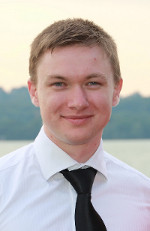
\includegraphics{photo.jpg}}
\ecvname{Sebastian Banescu}
%\ecvfootername{Sebastian Banescu \quad Date:~16.12.2014}
\ecvaddress{Hochbr\"{u}cker Weg 2, 85396 Eching, Germany}
\ecvtelephone{(+49) 176 4152 5239}
\ecvemail{banescusebi@gmail.com}
%\ecvhomepage{\href{https://www22.in.tum.de/banescu}{www22.in.tum.de/banescu}}
\ecvlinkedin{\href{https://de.linkedin.com/in/sebastianbanescu}{de.linkedin.com/in/sebastianbanescu}}
%\ecvdateofbirth{20 October 1987}
%\ecvgender{Male}
\ecvpicture[width=1.5cm]{photo.jpg}
%\ecvfootnote{For more information go to \url{http://europass.cedefop.eu.int}\\
%\textcopyright~European Communities, 2003.}

\begin{document}
\selectlanguage{english}

\begin{europecv}
\ecvpersonalinfo[10pt]
%\ecvitem{\large\textbf{Desired employment/ Occupational~field}}{\large\textbf{}}

\ecvsection{Education and Training}
\ecvitem{Dates}{October 2014 - April 2017}
\ecvitem{Position}{\textbf{PhD. student}}
\ecvitem{Name of organization}{\textbf{Technical University of Munich, Germany}, Center for Doctoral Studies in Informatics and its Applications (CeDoSIA) Graduate School, Faculty of Informatics}
\ecvitem{PhD. Thesis Title}{Characterizing the Strength of Software Obfuscation Against Automated Attacks}
\ecvitem{}{}
\ecvitem{Dates}{September 2010 - August 2012}
\ecvitem{Title of qualification awarded}{\textbf{MSc. Computer Science and Engineering - Information Security Technology} graduated \textit{``cum laude''} (GPA: 8.5 of 10, Thesis: 9 of 10)}
%\ecvitem{Principal subjects/Occupational skills covered}{Theoretical and technical expertise in the area of digital communication in general and in information security technology in particular.}
\ecvitem{Scholarship}{Talent Scholarship Program, currently Amandus H. Lundqvist Scholarship Program}
\ecvitem{Name of organization}{\textbf{Technical University of Eindhoven, The Netherlands}, Faculty of Computer Science}
\ecvitem{MSc. Thesis Title}{Decision support for privacy auditing}
\ecvitem{}{}
\ecvitem{Dates}{October 2006 - July 2010}
\ecvitem{Title of qualification awarded}{\textbf{BSc. Computer Science and Engineering} (GPA: 9.5 of 10, Thesis: 10 of 10)}
%\ecvitem{Principal subjects/Occupational skills covered}{The study and design of computer and network systems components from both hardware and software perspectives and multiple specialization alternatives such as: computer architecture design, software engineering, artificial intelligence, operating systems, database design, compiler design, transactional systems, computer networks and distributed systems.}
\ecvitem{Scholarship}{Merit-based and Performance-based scholarships due to academic results}
\ecvitem{Name of organization}{\textbf{Technical University of Cluj-Napoca, Romania}, Faculty of Computer Science}
\ecvitem{BSc. Thesis Title}{Unpredictable Random Number Generator Applied in Hardware Resource Allocation}
\ecvitem{}{}

\ecvsection{Research Visits}
\ecvitem{Dates}{February-March 2016}
\ecvitem{Position}{\textbf{Visiting Research Scholar} worked with Prof.~Dr.~Saumya Debray and Prof.~Dr.~Christian Collberg on characterizing obfuscation strength via case-studies using ELF x86 binaries.}
%\ecvitem{Principal subjects/Occupational skills covered}{Study and implement FPGA target abstractions for Altera Stratix II, III \& IV and Virtex 5. Devise, implement and test an arithmetic operator optimized for the Stratix architectures. All contributions are part of the FloPoCo Arithmetic Core Generator.}
\ecvitem{Name of organization}{\textbf{University of Arizona, Tucson, USA}, Faculty of Computer Science}
\ecvitem{}{}

\ecvitem{Dates}{September 2015}
\ecvitem{Position}{\textbf{Visiting Research Scholar} worked with Prof.~Dr.~Vijay Ganesh on employing symbolic execution and SAT/SMT solvers for the purpose of de-obfuscating ELF x86 binaries.}
%\ecvitem{Principal subjects/Occupational skills covered}{Study and implement FPGA target abstractions for Altera Stratix II, III \& IV and Virtex 5. Devise, implement and test an arithmetic operator optimized for the Stratix architectures. All contributions are part of the FloPoCo Arithmetic Core Generator.}
\ecvitem{Name of organization}{\textbf{University of Waterloo, Canada}, Department of Electrical and Computer Engineering}
\ecvitem{}{}

\ecvitem{Dates}{June 2009 - September 2009}
\ecvitem{Position}{\textbf{ERASMUS Exchange student} worked with Prof. Dr. Florent de Dinechin. Developed a high precision multiplication operators for FPGA chips. Mainly used C/C++ to generate VHDL.}
%\ecvitem{Principal subjects/Occupational skills covered}{Study and implement FPGA target abstractions for Altera Stratix II, III \& IV and Virtex 5. Devise, implement and test an arithmetic operator optimized for the Stratix architectures. All contributions are part of the FloPoCo Arithmetic Core Generator.}
%\ecvitem{Scholarship}{European Region Action Scheme for the Mobility of University Students (\small{ERASMUS})}
\ecvitem{Name of organization}{\textbf{Ecole Normale Superieure Lyon, France}, Laboratoire de l'Informatique du Parallélisme}
%\ecvitem{Level in national or international classification\footnote{If appropriate.}}{\ldots}
%\ecvitem{Dates}{2002 - 2006}
%\ecvitem{Title of qualification awarded}{High School Degree}
%\ecvitem{Principal subjects/Occupational skills covered}{The study of basic computer programming, database design and use of  Microsoft Office Suite and Microsoft Windows Operating System.}
%\ecvitem{Scholarship}{Merit-based due to high scores during entire period of studies}
%\ecvitem{Name and type of organization providing education and training}{Colegiul National "Mihai Eminescu", Satu Mare}
\ecvitem{}{}

\ecvsection{Work Experience}
\ecvitem{Dates}{May 2017 - onward}
\ecvitem{Position}{\textbf{IT Security Specialist} - member of Connected Security Team}
\ecvitem{Employer}{\textbf{BMW AG, Germany} - IT-Zentrum M\"unchen}
\ecvitem{Responsibilities}{Developing IT defenses against hackers, for the connected BMW cars.}
\ecvitem{}{}


\ecvitem{Dates}{April 2013 - April 2017}
\ecvitem{Position}{\textbf{Researcher / Teaching Assistant} - member of Software Engineering Chair}
\ecvitem{Employer}{\textbf{Technical University of Munich, Germany} - Faculty of Informatics}
\ecvitem{Responsibilities}{Research in the field of software protection, collaborated with Google Chrome security teams, developed solutions against browser hijacking malware in C/C++. Teaching assistance for MSc.~and BSc.~level courses, for 6 semesters. Co-developed ``Secure Coding'' lecture, which was awarded the TUM prize for teaching excellence. Advised over 15 MSc.~and BSc.~theses, many of which concluded with peer-reviewed publications; more details at https://www22.in.tum.de/banescu}
\ecvitem{}{}
\ecvitem{Dates}{September 2012 - March 2013}
\ecvitem{Position}{\textbf{Security Engineer} - member of Digital Video Broadcast team}
\ecvitem{Employer}{\textbf{TP Vision, The Netherlands} - Innovation Site Eindhoven}
\ecvitem{Responsibilities}{Secure design, integration and testing of key management, DRM, copy and content protection systems. 
Developed specifications for ARM TrustZone integration of the afore mentioned systems. Mainly used C/C++. Assessed compliance and robustness rules for new systems.}
\ecvitem{}{}
\ecvitem{Dates}{February 2012 - August 2012}
\ecvitem{Position}{\textbf{Master Thesis Intern} - member of the T-Clouds project team}
\ecvitem{Employer}{\textbf{Philips Research, The Netherlands} - Healthcare Information Management, Security Cluster}
\ecvitem{Responsibilities}{Developed secure logging and log aggregation module for the TClouds project co-financed
under EU FP7 and obtained \textbf{patent US20160134495} for it.
Developed a privacy infringement detection and quantification tool and published 2 peer-reviewed papers about it. Mainly used Java.}
\ecvitem{}{}
\ecvitem{Dates}{July 2011 - November 2011}
\ecvitem{Position}{\textbf{Intern Student} - member of Security \& Privacy team}
\ecvitem{Employer}{\textbf{Deloitte, The Netherlands} - Enterprise Risk Services}
\ecvitem{Responsibilities}{Manual and (semi-)automated penetration testing of web-applications. Developed a privacy escalation 
testing tool as a script for OWASP WebScarab. Developed a password brute-forcing script for iMacros FF and IE plug-in. Mainly used PHP.}
%\ecvitem{}{}
%\ecvitem{Dates}{2005 - 2008}
%\ecvitem{Occupation}{\textbf{Freelance Web Developer}}
%\ecvitem{Main activities}{Design and develop presentation and e-commerce websites. Technologies used: PHP, JavaScript, AJAX, HTML, CSS, MySQL, Joomla, Drupal, OpenCart, ZenCart, Magento, PrestaShop. \textbf{Rent-a-coder/V-worker account name: sk8er} (ranked higher than 96\% of peers).}

\ecvsection{Projects}

\ecvitem{Title}{\textbf{Symbolic Execution for Software Deobfuscation}}
\ecvitem{Description}{
Generated a set of over 5000 C program benchmarks and obfuscated them with various techniques, i.e.: self-modifying code, virtualization (emulation/packing), control-flow flattening, opaque predicates, mixed boolean-arithmetic, etc. 
Compiled programs using LLVM Clang and GCC into ELF binaries.
Recovered hidden passwords from obfuscated programs by applying directed dynamic symbolic execution on all obfuscated binaries.
Analyzed the effect of different obfuscation techniques on the effort required by the symbolic execution-based attack.
Identified major differences between different obfuscation transformations.}
\ecvitem{Skills Used}{Dynamic symbolic execution, software obfuscation, statistical analysis.}
\ecvitem{Technologies Used}{C, Python, Bash Script, R.}
\ecvitem{Achievements}{\textbf{Outstanding paper} at 32nd Annual Computer Security Applications Conference (ACSAC), 2016. Released dataset of over 5000 C programs to public to advance state of the art in software deobfuscation.}

\ecvitem{}{}
\ecvitem{Title}{\textbf{Machine Learning for Classification of Obfuscated Software}}
\ecvitem{Description}{
Created a dataset of over 11.000 obfuscated C programs and compiled them to ELF binaries. 
Extracted term-frequency inverse document-frequency (TF-IDF) features from artifacts resulting from both static and dynamic analysis of obfuscated ELF binaries.
Applied naive Bayes and decision tree classifiers to determine the obfuscation transformations applied on the obfuscated binaries.
Obtained 99\% classification accuracy of obfuscated binaries according to applied obfuscation transformations.}
\ecvitem{Skills Used}{Supervised machine learning for multi-level classification, static and dynamic binary analysis.}
\ecvitem{Technologies Used}{C, Python, Bash Script.}
\ecvitem{Achievements}{\textbf{Best paper} at 6th Software Security, Protection and Reverse Engineering Workshop (SSPREW), 2016. \textbf{Open source} implementation of binary analysis framework called Oedipus for metadata recovery.}

\ecvitem{}{}
% \ecvitem{Title}{\textbf{Machine Learning for Malware Analysis}}
% \ecvitem{Description}{
% Created tool to dynamically obfuscate real-world malware binaries.
% Extracted features from system call traces via sliding-window, from each obfuscated malware sample in the dataset.
% Performed 10-fold cross-validation of Support Vector Machines (SVMs) model for classifying malicious and benign software binaries.
% Determined that system call insertion based obfuscation is able to decrease accuracy of SVM model based on sliding windows.
% }
% \ecvitem{Skills Used}{Dynamic binary instrumentation, supervised machine learning for binary classification.}
% \ecvitem{Technologies Used}{C, Python.}
% \ecvitem{Achievements}{\textbf{Open source} implementation of behavior obfuscator called FEEBO. Peer-reviewed publication at 10th International Conference on Malicious and Unwandted Software (MALWARE), 2015.}
% 
% \ecvitem{}{}
\ecvitem{Title}{\textbf{Software-based Integrity Protection for Google Chrome}}
\ecvitem{Description}{
Wrote proposals and obtained grants for 2 projects in collaboration with Google Germany and Google Canada for developing software-based solutions for protecting Google Chrome against an instance of potentially unwanted programs called browser hijackers.
Developed solutions using white-box cryptography, control-flow integrity and dynamic code checksumming.
The solutions are able to protect both static and dynamic memory of Google Chrome against unwanted modifications by browser hijackers.
}
\ecvitem{Skills Used}{Software protection techniques, reverse engineering}
\ecvitem{Technologies Used}{C/C++, x86 Assembly}
\ecvitem{Achievements}{\textbf{Open source} implementation of software protection for Google Chrome. Two peer-reviewed publications at 5th and 7th ACM Conference on Data and Application Security and Privacy \newline (CODASPY), 2015 and 2017.}

\ecvsection{Peer-Reviewed Publications}
\ecvitem{1}{\textbf{Banescu, S}; Collberg, C; Pretschner, A; \textit{Predicting the Resilience of Obfuscated Code Against Symbolic Execution Attacks via Machine Learning}. To appear in Proc.~of the USENIX Security Symposium (USENIX Sec), 2017}
\ecvitem{2}{\textbf{Banescu, S}; Ahmadvand, M; Pretschner, A; \textit{Detecting Patching of Executables without System Calls}. In Proc.~of the 7th ACM Conference on Data and Application Security and Privacy (CODASPY), 2017}
\ecvitem{3}{Ochoa, M; \textbf{Banescu, S}; Disenfeld, C; Barthe, G; Ganesh, V; \textit{Reasoning about Probabilistic Defense Mechanisms against Remote Attacks.} In Proc.~of  2nd IEEE European Symposium on Security and Privacy (EuroS\&P), 2017}
\ecvitem{4}{\textbf{Banescu, S}; Collberg, C; Ganesh, V; Newsham, Z; Pretschner, A; \textit{Code Obfuscation Against Symbolic Execution Attacks.} In Proc.~of 32nd Annual Computer Security Applications Conference (ACSAC), 2016 \textbf{\color{red} Outstanding Paper Award}}
\ecvitem{5}{Salem, A; \textbf{Banescu, S}. \textit{Metadata Recovery From Obfuscated Programs Using Machine Learning}. In Proc.~of the 6th Software Security, Protection and Reverse Engineering Workshop (SSPREW@ACSAC), 2016 \textbf{\color{red}Best Paper Award}}
\ecvitem{6}{\textbf{Banescu, S}; Lucaci, C; Kr\"amer, B; Pretschner, A; \textit{VOT4CS: A Virtualization Obfuscation Tool for C\#}. In Proc.~of 2nd International Workshop on Software Protection (SPRO@CCS), 2016}
\ecvitem{7}{Ibrahim, A; \textbf{Banescu, S}; \textit{StIns4CS: A State Inspection Tool for C\#}. In Proc.~of 2nd International Workshop on Software Protection (SPRO@CCS), 2016}
\ecvitem{8}{Holling, D; \textbf{Banescu, S}; Probst, M; Petrovska, A; Pretschner, A; \textit{Nequivack: Assessing mutation score confidence}. In Proc.~of 9th International Conference on Software Testing, Verification and Validation Workshops (ICSTW), 2016}
\ecvitem{9}{\textbf{Banescu, S}; Wuechner, T; Salem, A; Guggenmos, M; Ochoa, M; Pretschner, A; \textit{A Framework for Empirical Evaluation of Malware Detection Resilience Against Behaviour Obfuscation}. In Proc.~of 10th International Conference on Malicious and Unwandted Software (MALWARE), 2015}
\ecvitem{10}{Fedler, R; \textbf{Banescu, S}; Pretschner, A; \textit{ISA2R: Improving Software Attack and Analysis Resilience via Compiler-Level Software Diversity}. In Proc.~of 34th International Conference on Safety, Reliability, and Security (SAFECOMP), 2015}
\ecvitem{11}{Ganesh, V; \textbf{Banescu, S}; Ochoa, M; \textit{The Meaning of Attack Resistant Systems}.
In Proc.~of the 10th Workshop on Programming Languages Analysis for Security (PLAS@ECOOP), 2015}
\ecvitem{12}{\textbf{Banescu, S}; Ochoa, M; Pretschner, A; \textit{A Framework for Measuring Software Resilience Against Automated Attacks}. In Proc.~of the 1st International Workshop on Software Protection (SPRO@ICSE), 2015}
\ecvitem{13}{\textbf{Banescu, S}; Pretschner, A; Battre, D; Cazzulani, S; Shield, R; Thompson, G; \textit{Software-Based Protection against ``Changeware''}. In Proc.~of the 5th ACM Conference on Data and Application Security and Privacy (CODASPY), 2015}
\ecvitem{14}{\textbf{Banescu, S}; Ochoa, M; Kunze, N; Pretschner, A; \textit{Idea: Benchmarking indistinguishability obfuscation - A candidate implementation}. In Proc.~of the International Symposium on Engineering Secure Software and Systems (ESSoS), 2015}
\ecvitem{15}{\textbf{Banescu, S}; Petkovic, M; Zannone, N; \textit{Measuring Privacy Compliance Using Fitness Metrics}. Proc.~of the 10th International Conference on Business Process Management (BPM), 2012}
\ecvitem{16}{Pieters, W; \textbf{Banescu, S}; Posea, S; \textit{Preventing system abuse by service composition}. Proc.~of the Third International Engineering Systems Symposium (CESUN), 2012}
\ecvitem{17}{\textbf{Banescu, S}; Zannone, N; \textit{Measuring privacy compliance with process specifications}. Proc.~of the 7th International Workshop on Security Measurements and Metrics (MetriSec), 2011}
\ecvitem{18}{Suciu, A; \textbf{Banescu, S}; Marton, K; \textit{Unpredictable random number generator based on hardware performance counters}. Digital Information Processing and Communications, 2011}
\ecvitem{19}{\textbf{Banescu, S}; de Dinechin, F; Pasca, B; Tudoran R; - \textit{Multipliers for Floating-Point Double Precision and Beyond on FPGAs}.
Proc.~of the 1st International Workshop on Highly Efficient Accelerators and Reconfigurable Technologies (HEART), 2010}
\ecvitem{20}{Tudoran, R; \textbf{Banescu, S}; Cret, O; Suciu, A; - \textit{Implementing True Random Number Generators by Overfilling the FPGA Chip}. Proc.~of the FPGA World 2009 International Conference, 2009}
\ecvitem{21}{Colesa, A; Tudoran, R; \textbf{Banescu, S} - \textit{Software Random Number Generation Based on Race Conditions}. Proc.~of the 10th International Symposium on Symbolic and Numeric Algorithms for Scientific Computing, September (SYNASC), 2008}
%\ecvitem{7}{Saplacan, G; Buzdugan, L.; Rusu, M.; Salomie, I.; Nedevschi, S.; Dinsoreanu, M.; Sebestyen, G.; Alban, C.; \textbf{Banescu, S.}; Daian, A.; Gasko, T.; Ghirisan, A.; Gorcea, I.; Tudoran, R.; Turian, V. - \textbf{Resource Configuration Tools for a Traceability System in Food Industry}. Proc.~of the Workshop on Traceability and Systems for Traceability, IEEE International Conference on Intelligent Computer Communication and Processing, August, 2008, Cluj-Napoca, Romania, pp 29, ISBN 978-973-133-358-82008}

\ecvsection{Personal Skills and~Competences}
\ecvmothertongue[5pt]{Romanian}
\ecvlanguageheader{}
\ecvlanguage{English}{\footnotesize{Advanced (C2)}}{\footnotesize{Advanced (C2)}}{\footnotesize{Advanced (C1)}}{\footnotesize{Advanced (C1)}}{\footnotesize{Advanced (C1)}}
\ecvlanguage{German}{\footnotesize{Intermediate (B2)}}{\footnotesize{Intermediate (B2)}}{\footnotesize{Intermediate (B1)}}{\footnotesize{Intermediate (B1)}}{\footnotesize{Intermediate (B1)}}
%\ecvlanguage{Dutch}{\footnotesize{Beginner (A2)}}{\footnotesize{Beginner (A2)}}{\footnotesize{Beginner (A1)}}{\footnotesize{Beginner (A1)}}{\footnotesize{Beginner (A1)}}
%\ecvlanguagefooter[5pt]{(*)}
\ecvitem{}{}
\ecvitem{Programming and}{\emph{Intermediate: } Java, C, R, x86 Assembly, Bash Script, C++, Python}
\ecvitem{Scripting Languages}{\emph{Beginner: } C\#, VHDL, Matlab, Prolog, Haskel, ML, Lisp \vspace{0.2cm}}
\ecvitem{Web Technologies}{\emph{Intermediate:} PHP, HTML, JavaScript, CSS, AJAX, XML
\vspace{0.2cm}}
\ecvitem{Black-Box Testing Tools}{\emph{Beginner:} Nessus, Burpsuite, ZAP, Wireshark, Sqlmap, Zenmap
\vspace{0.2cm}}
\ecvitem{White-Box Testing Tools}{\emph{Intermediate:} KLEE, S2E} \ecvitem{}{\emph{Beginner:} Fortify, RIPS, FindBugs
\vspace{0.2cm}}
\ecvitem{Reverse Engineering}{\emph{Intermediate:} IDA Pro, GDB, angr, Triton, JavaDecompiler
\vspace{0.2cm}}
\ecvitem{Integrated Development}{\emph{Intermediate:} Eclipse, MS Visual Studio}
\ecvitem{Environments}{\emph{Beginner:} vim, Matlab, Xilinx ISE
\vspace{0.2cm}}
\ecvitem{SCM Tools}{\emph{Intermediate:} Subversion (SVN), Git
\vspace{0.2cm}}
\ecvitem{DBMS\vspace{0.3cm}}{\emph{Intermediate:} MySQL, MS SQL Server
\vspace{0.2cm}}
%\ecvitem{Operating Systems}{Linux Debian/Ubuntu, Windows, Android
%\vspace{0.2cm}}
%\ecvitem{Document Editing Software}{LaTeX editors WinEdt and Kile; Microsoft Office Suite; Open/Libre Office Suite
%\vspace{0.2cm}}

\ecvitem{Soft Skills}{Great Communication Skills, Team Player, Detail Oriented, Public Speaking \& Presenting}

\ecvsection{Miscellaneous}
\ecvitem{\large Activities and Achievements}{Contributer to \textbf{Google Syzygy} open source project https://github.com/banescusebi
\vspace{0.1cm}}
%\ecvitem{-}{Member of the ``kopipacket'' team comprising of researchers at the Technical University of Munich and the Singapore University of Technology and Design, which regularly achieves \textbf{top 5\% rankings in capture the flag (CTF) competitions} \vspace{0.1cm}}
\ecvitem{-}{\textbf{Outstanding paper award} at 32nd Annual Computer Security Applications Conference \newline (ACSAC), December 2016\vspace{0.1cm}}
\ecvitem{-}{\textbf{Best paper award} at 6th Software Security, Protection and Reverse Engineering Workshop (SSPREW), December 2016\vspace{0.1cm}}
\ecvitem{-}{\textbf{Invited speaker} at Itestra GmbH Jour Fixe, December 2016, Munich Germany \vspace{0.1cm}}
\ecvitem{-}{\textbf{Invited speaker} at Friedrich-Alexander Universit\"{a}t (FAU) Erlangen by Prof.~Dr.-Ing.~Felix Freiling, September 2016, Erlangen Germany. \vspace{0.1cm}}
\ecvitem{-}{\textbf{Invited trainer} at ``Software Protection Workshop'' organized by Dolby Germany, August 2016}
\ecvitem{-}{\textbf{Winner of ``Best Code Cracker of ISSISP 2014''} award at the International Summer School on Information Security and Protection, July 2014, Verona, Italy
\vspace{0.1cm}}
\ecvitem{-}{Participated in various \textbf{mathematics and informatics olympiads and contests} at county and national levels. Obtained notable awards including \textbf{1st, 2nd and 3rd prizes} (1998-2006)
\vspace{0.1cm}}
\ecvitem{\large Volunteer Work}{Volunteer IT Consultant for League of Romanian Students Abroad (2010-2012)
\vspace{0.1cm}}
 %\item Microsoft .NET Summer Rally in 2008 organized by Microsoft Student Partners in Cluj-Napoca.
\ecvitem{}{Volunteer in civic cleaning campaigns in my home town (1998-2006)
\vspace{0.2cm}}

\ecvitem{\large Recommendations}{Upon request from Prof.~Dr.~Alexander Pretschner, e-mail: alexander.pretschner@tum.de}
\ecvitem{}{Other 10 recommendations already available on Linkedin: de.linkedin.com/in/sebastianbanescu}
\ecvitem{\large Hobbies}{Snowboarding, Football, Hiking, Board games
\vspace{0.2cm}}

%\ecvitem{\large Other interests}{Data Science, Psychology, Advertising}

%\ecvitem{\large Driver's license}{Category B, Since: 29 November 2005}

\end{europecv}


\end{document} 